\pdfminorversion=4
\documentclass[compress,
mathserif,wide,%red,
%handout
]{beamer}

\usepackage{amsmath,amsfonts,bm,bbm,comment}
\usepackage{latexsym,tabularx,amscd}
\usepackage{etex} 
\usepackage{algorithm}
\usepackage[noend]{algorithmic}
\usepackage{subfigure}
\usepackage{url}
%\usepackage{multimedia}
\usepackage{hyperref}
\usepackage{skull}
%\usepackage{enumitem}
%\usepackage{movie15}

\usepackage{multirow}
\usepackage{cancel}

%\usepackage{ulem}
\usepackage{lmodern}
\usepackage{array} 
\usepackage{etoolbox}
\usepackage{caption}
\usepackage[normalem]{ulem}

\usepackage{mathtools}

\usepackage[space]{grffile}

\usepackage{tikz}
\usetikzlibrary{shapes.arrows}
\usetikzlibrary{arrows,positioning}
\usepackage{pgfplots}
%\usetikzlibrary{pgfplots.groupplots}

\tikzset{
    myarrow/.style={
        draw,
        fill=black,
        single arrow,
        minimum height=6ex,
        single arrow head extend=1ex
    }
}


\newcommand{\vertiii}[1]{{\left\vert\kern-0.25ex\left\vert\kern-0.25ex\left\vert #1 
    \right\vert\kern-0.25ex\right\vert\kern-0.25ex\right\vert}}

\newcommand{\vertiiibig}[1]{{\big\vert\kern-0.25ex\big\vert\kern-0.25ex\big\vert #1 
    \big\vert\kern-0.25ex\big\vert\kern-0.25ex\big\vert}}

\newcommand{\vertiiiplain}[1]{{\vert\kern-0.25ex\vert\kern-0.25ex\vert #1 
    \vert\kern-0.25ex\vert\kern-0.25ex\vert}}



\usepackage{dsfont}
\DeclareMathOperator{\ind}{\mathds{1}}  % Indicator


\newcommand{\abs}[1]{\left|#1\right|}

\mode<presentation>

\usetheme{Madrid}
% other themes: AnnArbor, Antibes, Bergen, Berkeley, Berlin, Boadilla,
% boxes, CambridgeUS, Copenhagen, Darmstadt, default, Dresden,
% Frankfurt, Goettingen, Hannover, Ilmenau, JuanLesPins, Luebeck,
% Madrid, Maloe, Marburg, Montpellier, PaloAlto, Pittsburg, Rochester,
% Singapore, Szeged, classic

% \usecolortheme{lily} 
% color themes: albatross, beaver, beetle, crane, default, dolphin,
% dov, fly, lily, orchid, rose, seagull, seahorse, sidebartab,
% structure, whale, wolverine

% \usefonttheme{serif} 
% font themes: default, professionalfonts, serif, structurebold,
% structureitalicserif, structuresmallcapsserif

%\usefonttheme[onlymath]{serif}
%\usefonttheme[onlylarge]{structuresmallcapsserif} 
  
%\useoutertheme[subsection=false]{smoothbars}
% outer themes:
% default,infolines,miniframes,smoothbars,sidebar,split,shadow,tree,smoothtree
%\useinnertheme{rectangles}
\beamertemplatenavigationsymbolsempty

% \definecolor{fore}{RGB}{249,242,215}
% \definecolor{back}{RGB}{51,51,51}
% \definecolor{title}{RGB}{255,0,90}
% \setbeamercolor{titlelike}{fg=title}
% \setbeamercolor{normal text}{fg=fore,bg=back}
% \setbeamercovered{transparent}
  % or whatever (possibly just delete it)
%\beamertemplatenavigationsymbolsempty

\usepackage[english]{babel}
\usepackage[latin1]{inputenc}
% or whatever
%\usepackage{comicsans} 
%\renewcommand{\sfdefault}{comic} 
%\usepackage{mathptmx}
%\mathversion{bold}
%\usepackage{helvet}
%\usepackage{courier}

%\usepackage[T1]{fontenc}
% Or whatever. Note that the encoding and the font should match. If T1
% does not look nice, try deleting the line with the fontenc.


%%%% Figures %%%%%


\newcommand{\LectureFigs}{../Figures}


\definecolor{bluegray}{rgb}{0.15,0.20,0.40}
\definecolor{bluegraylight}{rgb}{0.35,0.40,0.60}
\definecolor{gray}{rgb}{0.3,0.3,0.3}
\definecolor{lightgray}{rgb}{0.7,0.7,0.7}
\definecolor{brightblue}{rgb}{0.1,0.4,0.7}
\definecolor{darkblue}{rgb}{0.1,0.1,0.6}
\definecolor{darkgreen}{rgb}{0.0,0.5,0.2}
\definecolor{orange}{rgb}{0.7,0.3,0}

\def \captioncolor { }

\setbeamertemplate{itemize item}{{\color{black}$\bullet$}}
\setbeamertemplate{itemize subitem}{{\color{black}$\circ$}}
\setbeamertemplate{frametitle}[default][center]
\setbeamerfont{frametitle}{series=\bfseries}
\addtobeamertemplate{frametitle}{\vskip1ex}{ \vspace{0.5em} \hrule}
\setbeamercolor{frametitle}{fg=,bg=}

\setbeamertemplate{theorems}[numbered]
\setbeamertemplate{caption}[numbered]
\setbeamertemplate{algorithm}[numbered]

\numberwithin{theorem}{subsection}
\numberwithin{equation}{subsection}
\numberwithin{figure}{subsection}
\numberwithin{algorithm}{subsection}


%\setbeamerfont{page number in head/foot}{size=\scriptsize}
\setbeamertemplate{footline}[frame number]
\setbeamercolor{page number in head/foot}{fg=black}
\setbeamersize{text margin left=2em,text margin right=2em}

\setbeamertemplate{footline}
{
    %\hspace{3em} \insertshorttitle \hfill \insertframenumber / \inserttotalframenumber\hspace{3em}
    \hspace{3em} \insertshorttitle \hfill \insertsubsectionnumber-\insertframenumber \hspace{3em}
    \vspace{1.5em}
}

\definecolor{babyblueeyes}{rgb}{0.63, 0.79, 0.95}
\definecolor{bleudefrance}{rgb}{0.19, 0.55, 0.91}
\definecolor{matlabPlotBlue}{rgb}{0.25, 0.58, 0.8}
\definecolor{matlabPlotOrange}{rgb}{0.855, 0.324, 0.098}



\captionsetup[figure]{labelfont={color=black}}

\AtBeginEnvironment{lemma}{%
  \setbeamercolor{block title}{fg=black,bg=babyblueeyes}
  \setbeamercolor{block body}{fg=black,bg=}
  \setbeamerfont*{block title}{series=\bfseries}
}

\AtBeginEnvironment{theorem}{%
  \setbeamercolor{block title}{fg=black,bg=babyblueeyes}
  \setbeamercolor{block body}{fg=black,bg=}
  \setbeamerfont*{block title}{series=\bfseries}
}

\AtBeginEnvironment{corollary}{%
  \setbeamercolor{block title}{fg=black,bg=babyblueeyes}
  \setbeamercolor{block body}{fg=black,bg=}
  \setbeamerfont*{block title}{series=\bfseries}
}

\AtBeginEnvironment{fact}{%
  \setbeamercolor{block title}{fg=black,bg=babyblueeyes}
  \setbeamercolor{block body}{fg=black,bg=}
  \setbeamerfont*{block title}{series=\bfseries}
}

\AtBeginEnvironment{definition}{%
  \setbeamercolor{block title}{fg=black,bg=babyblueeyes}
  \setbeamercolor{block body}{fg=black,bg=}
  \setbeamerfont*{block title}{series=\bfseries}
}

\newenvironment<>{varblock}[2][.9\textwidth]{%
  \vspace{-1em}
  \begin{center}
  \begin{minipage}{#1}
  %\setlength{\textwidth}{#1}
  \begin{actionenv}#3%
    \def\insertblocktitle{#2}%
    \par%
    \usebeamertemplate{block begin}}
  {\par%
    \usebeamertemplate{block end}%
  \end{actionenv}
  \end{minipage}
  \end{center}
}


\newcommand\blankfootnote[1]{%
  \let\thefootnote\relax\footnotetext{#1}%
  \let\thefootnote\svthefootnote%
}


%%%%%
\newcommand{\bb}{\bm b}
\newcommand{\bZ}{\bm Z}
\newcommand{\bC}{\bm C}
\newcommand{\cU}{{\cal U}}
\newcommand{\bR}{{\bm R}}
\newcommand{\bi}{{\bm i}}
\newcommand{\bS}{{\bm S}}
\newcommand{\cE}{{\cal E}}
\newcommand{\cF}{{\cal F}}
\newcommand{\bk}{{\bm k}}
\newcommand{\bu}{{\bm u}}
\newcommand{\bx}{{\bm x}}
\newcommand{\bA}{{\bm A}}
\newcommand{\bh}{{\bm h}}
\newcommand{\by}{{\bm y}}
\newcommand{\bI}{{\bm I}}
\newcommand{\ba}{{\bm a}}
\newcommand{\bw}{{\bm w}}
\newcommand{\bPhi}{{\bm \Phi}}
\newcommand{\bX}{{\bm X}}
\newcommand{\bY}{{\bm Y}}
\newcommand{\bM}{{\bm M}}
\newcommand{\be}{{\bm e}}
\newcommand{\bs}{{\bm s}}
\newcommand{\bB}{{\bm B}}
\newcommand{\bW}{{\bm W}}
\newcommand{\bN}{{\bm N}}
\newcommand{\bU}{{\bm U}}
\newcommand{\bV}{{\bm V}}
\newcommand{\bP}{{\bm P}}
\newcommand{\bH}{{\bm H}}
\newcommand{\bSigma}{{\bm \Sigma}}
\newcommand{\bL}{{\bm L}}



\newcommand{\bv}{\bm v}
\newcommand{\eps}{\epsilon}
\newcommand{\vf}{\varphi}
\newcommand{\de}{\delta}
\newcommand{\<}{\langle}
\renewcommand{\>}{\rangle}
\newcommand{\goto}{\rightarrow}
\newcommand{\argmin}{\mbox{argmin}}
\newcommand{\argmax}{\mbox{argmax}}
\newcommand{\Ave}{\mathop{\rm Ave}\nolimits}
\newcommand{\sgn}{\mbox{sgn}}
\newcommand{\cN}{\mathcal{N}}
\newcommand{\cR}{\mathcal{R}}

\def\C{{\mathbb{C}}}
\def\R{{{\mathbb{R}}}} %seemed too large in subscripts, so I changed --JW 
\def\P{{\hbox{\bf P}}}
\def\Z{{{\mathbb{Z}}}}
\def\T{{\hbox{\bf T}}}


\newcommand{\cA}{\mathcal{A}}
\newcommand{\cP}{\mathcal{P}}
\newcommand{\cD}{\mathcal{D}}
\newcommand{\cL}{\mathcal{L}}
\newcommand{\shrink}{\text{shrink}}


\newcommand{\Obs}{\Omega_{\text{obs}}}


\renewcommand{\P}{\operatorname{\mathbb{P}}}
\newcommand{\E}{\operatorname{\mathbb{E}}}

% Linear algebra macros
%\newcommand{\vct}[1]{#1}
%\newcommand{\mtx}[1]{#1}
\newcommand{\vct}[1]{\bm{#1}}
\newcommand{\mtx}[1]{\bm{#1}}
%\newcommand{\mtx}[1]{\mathsfsl{#1}}

\newcommand{\transp}{T}
\newcommand{\adj}{*}
\newcommand{\psinv}{\dagger}
\newcommand{\lspan}[1]{\operatorname{span}{#1}}

\newcommand{\range}{\operatorname{range}}
\newcommand{\colspan}{\operatorname{colspan}}

\newcommand{\rank}{\text{rank}}

\newcommand{\diag}{\operatorname{diag}}
\newcommand{\trace}{\text{Tr}}

\newcommand{\supp}[1]{\operatorname{supp}(#1)}

\newcommand{\smax}{\sigma_{\max}}
\newcommand{\smin}{\sigma_{\min}}

\newcommand{\restrict}[1]{\big\vert_{#1}}

\newcommand{\Id}{\text{\em I}}
\newcommand{\OpId}{\mathcal{I}}



% define your own colors:
\definecolor{Red}{rgb}{1,0,0}
\definecolor{Blue}{rgb}{0,0,1}
\definecolor{Green}{rgb}{0,1,0}
\definecolor{magenta}{rgb}{1,0,.6}
\definecolor{lightblue}{rgb}{0,.5,1}
\definecolor{lightpurple}{rgb}{.6,.4,1}
\definecolor{gold}{rgb}{.6,.5,0}
\definecolor{orange}{rgb}{1,0.4,0}
\definecolor{hotpink}{rgb}{1,0,0.5}
\definecolor{newcolor2}{rgb}{.5,.3,.5}
\definecolor{newcolor}{rgb}{0,.3,1}
\definecolor{newcolor3}{rgb}{1,0,.35}
\definecolor{darkgreen1}{rgb}{0, .35, 0}
\definecolor{darkgreen}{rgb}{0, .6, 0}
\definecolor{darkred}{rgb}{.75,0,0}

\xdefinecolor{olive}{cmyk}{0.64,0,0.95,0.4}
\xdefinecolor{purpleish}{cmyk}{0.75,0.75,0,0}

\definecolor{lightgrey}{RGB}{186,186,186}
\definecolor{back}{RGB}{51,51,51}
\definecolor{fore}{RGB}{249,242,215}
\definecolor{back}{RGB}{51,51,51}
\definecolor{title}{RGB}{255,0,20}
\definecolor{keywords}{RGB}{255,0,90}
\definecolor{comments}{RGB}{60,179,113}
\definecolor{cobalt}{RGB}{102,153,204}

\def \itemstyle {\bf}
\def \itemhighlight {\bf}  

% \definecolor{blockbodycolor}{RGB}{30,30,40}
% \definecolor{blocktitlecolor}{RGB}{55,55,75}
\definecolor{blockbodycolor}{RGB}{186,206,232}
\definecolor{blocktitlecolor}{RGB}{55,55,75}

\setbeamercolor{titlelike}{fg=darkred,bg=white}
\setbeamercolor{normal text}{fg=black,bg=white}
\setbeamercolor{block title}{fg=white,bg=blocktitlecolor}
\setbeamercolor{block body}{bg=blockbodycolor}
\setbeamercolor{alerted text}{fg=darkred}
\setbeamercolor{title}{fg=darkred,bg=lightgrey}


\newcommand{\alertb}[1]{\textcolor{blue}{ #1}}

\newcommand{\yp}[1]{\textcolor{red}{ #1}}
\newcommand{\zeronorm}[1]{\left\|#1 \right\|_0}
\newcommand{\unorm}[1]{\left\|#1 \right\|_u}
\newcommand{\ynorm}[1]{\left\|#1 \right\|_{\bar{y}}}
\newcommand{\onetwonorm}[1]{\left\|#1\right\|_{1,2}}
\newcommand{\opnorm}[1]{\left\|#1\right\|}
\newcommand{\fronorm}[1]{\left\|#1\right\|_{F}}
\newcommand{\onenorm}[1]{\left\|#1\right\|_{\ell_1}}
\newcommand{\twonorm}[1]{\left\|#1\right\|_{2}}
\newcommand{\oneinfnorm}[1]{\left\|#1\right\|_{1,\infty}}
\newcommand{\infnorm}[1]{\left\|#1\right\|_{\ell_\infty}}
\newcommand{\nucnorm}[1]{\left\|#1\right\|_*}

%\makeatletter
%\def\th@mystyle{%
%    \normalfont % body font
%    \setbeamercolor{block title example}{bg=,fg=black}
%    \setbeamerfont{block title example}{series=\bfseries}
%    \setbeamercolor{block body example}{bg=,fg=black}
%    %\setbeamertemplate{exampleblock}[numbered]
%    \def\inserttheoremblockenv{exampleblock}
%  }
%\makeatother
%\theoremstyle{mystyle}
%\newtheorem*{lem}{Lemma}

\setbeamertemplate{frametitle continuation}{}


\newcommand{\courseTitle}{STAT 37797: Mathematics of Data Science} 



% \subtitle
% {Include Only If Paper Has a Subtitle}

\vspace{.5cm}

\author{Yuxin Chen}

\institute[Princeton] % (optional, but mostly needed)
{Princeton University}


% - Use the \inst command only if there are several affiliations.
% - Keep it simple, no one is interested in your street address.


\subject{Beamer}
% This is only inserted into the PDF information catalog. Can be left
% out.

% Delete this, if you do not want the table of contents to pop up at
% the beginning of each subsection:
% \AtBeginSubsection[]
% {
%   \begin{frame}<beamer>
%     \frametitle{Outline}
%     \tableofcontents[currentsection,currentsubsection]
%   \end{frame}
% }






\graphicspath{{../../../Figures/}}


\title % (optional, use only with long paper titles)
{Spectral methods: $\ell_{\infty}$ perturbation theory}

\defbeamertemplate*{title page}{customized}[1][]
{

  \hfill {\em \courseTitle}

  \begin{center}
    \vspace{2.5em}
    \usebeamerfont{title} {\Large\bf\inserttitle} \par
  
    \vspace{1.5em}
    \includegraphics[width=2cm]{\LectureFigs/UC_logo.png} 
  
    \vspace{1em}
    {\large Cong Ma \par }

    \vspace{0.2em}
    { \large \quad University of Chicago, Autumn 2021 }
  \end{center}

  \vfill
}

\setcounter{subsection}{6}

\begin{document}


\begin{frame}[plain]
  \titlepage

\end{frame}








\begin{frame}
	\frametitle{Revisit stochastic block model}

\vspace{-1em}


\begin{columns}

\begin{column}{0.05\textwidth}
\end{column}


\begin{column}{0.25\textwidth}
\begin{center}
  \includegraphics[height=0.9\textwidth]{SBM_1.png} \\
	$\mathcal{G}$
\end{center}
\end{column}

\begin{column}{0.05\textwidth}
\end{column}


\begin{column}{0.12\textwidth}
\begin{center}
\includegraphics[width=\textwidth,angle=-90]{arrow_up.png} 
\end{center}
\end{column}


\begin{column}{0.5\textwidth}
\begin{center}
  \includegraphics[height=0.45\textwidth]{SBM_2.png}
\end{center}
\end{column}

\begin{column}{0.03\textwidth}
\end{column}

\end{columns}


\bigskip


\begin{itemize}
	\itemsep0.5em
	\item Community membership vector \\
	$\qquad x_1^{\star}=\cdots=x_{n/2}^{\star}=1$; $x_{n/2+1}^{\star}=\cdots=x_n^{\star}=-1$ 
	\item observe a graph $\mathcal{G}$ (assuming $p>q$)
		\vspace{-0.5em}
		\begin{align*}
			(i,j)\in \mathcal{G} \text{ with prob.~} \begin{cases} p,  & \text{if }x_i = x_j \\ q, & \text{else} \end{cases}
		\end{align*}
	\item {\bf Goal:}  recover community memberships $\pm \bm{x}^\star$ 
\end{itemize}

\end{frame}



\begin{frame}
\frametitle{Revisit spectral clustering}

		
\begin{center}
\begin{tabular}{ccccc}
\includegraphics[width=0.23\textwidth,height=0.23\textwidth]{adjacency_random.png} &   & \includegraphics[width=0.23\textwidth,height=0.23\textwidth]{adjacency_mean.png} &  & \includegraphics[width=0.23\textwidth,height=0.23\textwidth]{adjacency_noise.png}\tabularnewline
	$\bm{A}$ & = & $\underset{\alertb{\text{rank 2}}}{\underbrace{\mathbb{E}[\bm{A}]}}$ & + & $\bm{A}-\mathbb{E}\left[\bm{A}\right]$\tabularnewline
\end{tabular}
\end{center}

\vspace{-0.5em}
\begin{itemize}
	\item[{\color{black}1.}] computing the leading eigenvector $\bm{u}=[u_i]_{1\leq i\leq n}$ of $\bm{A} - \frac{p+q}{2}\bm{1}\bm{1}^{\top}$
	\item[{\color{black}2.}] rounding:  output
		${x}_{i}=\begin{cases}
			1, & \text{if }u_{i} \geq 0\\
			-1, & \text{if }u_{i}<0
\end{cases}$
\end{itemize}

\end{frame}



\begin{frame}
\frametitle{Almost exact recovery}

\[
	\alert{\frac{p-q}{\sqrt{p}}\gg \sqrt{\frac{\log n}{n}}} \quad \Longrightarrow \quad \text{almost exact recovery} 
\]

\vfill 
\begin{itemize}
	\item Almost exact recovery means
	\[
	\min \left \{ \frac{1}{n}\sum_{i=1}^{n} \mathbbm{1} \big\{ x_{i}\neq x_{i}^{\star}\big\},  \frac{1}{n}\sum_{i=1}^{n} \mathbbm{1} \big\{ x_{i}\neq -x_{i}^{\star}\big\} \right \} = o(1)
	\]
\end{itemize}
\end{frame}

\begin{frame}
	\frametitle{Empirical performance of spectral clustering}
	\begin{figure}
	\includegraphics[width=0.6\textwidth]{SBM_experiment.pdf}
	\end{figure}
	
	
	{
\setbeamercolor{block body}{bg=babyblueeyes,fg=black}

\begin{varblock}[\textwidth]{}
\begin{center}
	$\ell_{2}$ perturbation theory alone cannot explain exact recovery guarantees
\end{center}
\end{varblock}
}
\hfill --- call for fine-grained analysis
	\end{frame}
	




\begin{frame}
	\frametitle{Reverse engineering}

\begin{columns}

\begin{column}{0.92\textwidth}
\begin{itemize}
  \item[] Spectral clustering uses signs of $\bm{u}$ to cluster nodes 
  \pause

  \vspace{-1em}
  \begin{figure}
	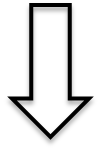
\includegraphics[width=0.05\textwidth,angle=180]{arrow_down_3.png} \qquad 
  \end{figure}

  \item[] It achieves exact recovery iff $u_{i} u_{i}^{\star} > 0$ for all $i$

  \pause
  \vspace{-1em}
  \begin{figure}
	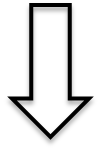
\includegraphics[width=0.05\textwidth,angle=180]{arrow_down_3.png} \qquad 
  \end{figure}


  \item[] A sufficient condition is\alertb{$^*$}  $\|\bm{u} - \bm{u}^{\star}\|_{\infty} < 1/\sqrt{n}$

  
  \uncover<4->{
  \vspace{-1em}
  \begin{figure}
	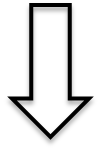
\includegraphics[width=0.05\textwidth,angle=180]{arrow_down_3.png}
  \end{figure}


  \item[] Need $\ell_{\infty}$ perturbation theory

  }
\end{itemize}



\end{column}
\end{columns}

\end{frame}


\begin{frame}
\frametitle{Outline}

\begin{itemize}
  \itemsep1em
  \item An illustrative example: rank-1 matrix denoising
  \item General $\ell_{\infty}$ perturbation theory: rank-1
  \item Application: exact recovery in community detection
  \item General $\ell_{2,\infty}$ perturbation theory: rank-r case
  \item Application: entrywise error in matrix completion
\end{itemize}

\end{frame}





\begin{frame}
	\frametitle{Setup and algorithm}
	
	\begin{itemize}
		\itemsep 0.5em
		\item Groundtruth: $\bm{M}^{\star} = \lambda^{\star} \bm{u}^{\star} \bm{u}^{\star\top}\in \mathbb{R}^{n\times n}$, with $\lambda^\star > 0$
		\item Observation: $\bm{M} = \bm{M}^{\star} + \bm{E}$, where $\bm{E}$ is symmetric, and its upper triangular part comprises of i.i.d.~$\mathcal{N}(0, \sigma^2)$ entries
		\item Estimate $\bm{u}^{\star}$ using $\bm{u}$, leading eigenvector of $\bm{M}$
		\item Goal: characterize entrywise errror
		 \begin{align*}
	\mathsf{dist}_{\infty}\big(\bm{u},\bm{u}^{\star}\big)
	\coloneqq \min\big\{ \|\bm{u}-\bm{u}^{\star}\|_{\infty}, \|\bm{u}+\bm{u}^{\star}\|_{\infty} \big\}
\end{align*}
	\end{itemize}


\end{frame}


\begin{frame}
	\frametitle{$\ell_{2}$ guarantees}
	
	We start with characterizing noise size
	 
	\begin{lemma}
	Assume symmetric Gaussian noise model. With high prob., one has
	\[
	\|\bm{E}\| \leq 5 \sigma \sqrt{n}
	\] 
	\end{lemma}
	
	\vfill 
	This in conjunction with Davis-Kahan's $\sin \bm{\Theta}$ theorem leads to: 
	\[
	\mathsf{dist}(\bm{u}, \bm{u}^{\star}) \leq \frac{2\| \bm{E} \|}{ \lambda^\star } \leq \frac{10\sigma \sqrt{n} }{ \lambda^\star},
	\]
	as long as $\sigma \sqrt{n} \leq \frac{1 - 1/\sqrt{2} }{5} \lambda^\star$ so that $\|\bm{E}\| \leq (1 - 1 / \sqrt{2}) \lambda^\star$
	
	\vfill 
	{\hfill \em \footnotesize --- implies $\mathsf{dist}_{\infty}\big(\bm{u},\bm{u}^{\star}\big) \leq \mathsf{dist}\big(\bm{u},\bm{u}^{\star}\big) \lesssim \frac{\sigma \sqrt{n} }{ \lambda }$  }
\end{frame}

\begin{frame}
	\frametitle{Incoherence}
	\begin{definition}
	Fix a unit vector $\bm{u}^\star \in \mathbb{R}^{n}$. Define its incoherence to be
	\begin{align*}
	\mu \coloneqq {n\|\bm{u}^{\star}\|_{\infty}^{2}} 
\end{align*}
\end{definition}

\vfill
\begin{itemize}
	\item Range of possible values of $\mu$: $1 \leq \mu \leq n$
	\item Two extremes: $\bm{u}^\star = \bm{e}_{1}$, and $\bm{u}^\star = (1 / \sqrt{n}) \cdot \bm{1}_{n}$
	\item Small $\mu$ indicates energy of eigenvector is spread across different entries
	\item Consider SBM and random Gaussian vectors
\end{itemize}

\end{frame}

\begin{frame}
	\frametitle{$\ell_{\infty}$ guarantees for matrix denoising}
	\begin{theorem}\label{thm:denoising-inf}
		Suppose that $\sigma \sqrt{n} \leq c_0 \lambda^\star$ for some sufficiently small constant $c_0 > 0$. Then whp., we have 
		\[
		\mathsf{dist}_{\infty} \big(\bm{u},\bm{u}^{\star}\big) \lesssim \frac{\sigma (\sqrt{\log n} + \sqrt{\mu} ) }{ \lambda^\star }
		\]
	\end{theorem}
	
	\begin{itemize}
		\item When $\mu \lesssim \log n$ (i.e., no entries are significantly larger than average), our bound reads
		\[
		\mathsf{dist}_{\infty} \big(\bm{u},\bm{u}^{\star}\big) \lesssim \frac{\sigma \sqrt{\log n} }{ \lambda^\star }
		\]
		\item Much tighter than $\ell_{2}$ bound: $\sqrt{ n / \log n}$ times smaller
	\end{itemize}
\end{frame}

\begin{frame}
	\frametitle{Technical hurdle: dependency}
	We would like to understand $u_{l}$. Since $\bm{u}$ is eigenvector of $\bm{M}$, we have
	\[
	\bm{M} \bm{u} = \lambda \bm{u},
	\]
	which yields 
	\begin{align*}
	u_l & = \frac{1}{\lambda} [\bm{M}]_{l, :} \bm{u} = \frac{1}{\lambda} [\bm{M}^{\star} + \bm{E} ]_{l, :} \bm{u} \\
	\end{align*}
	
{
\setbeamercolor{block body}{bg=babyblueeyes,fg=black}

\begin{varblock}[\textwidth]{}
\begin{center}
	$\bm{u}$ is dependent on $\bm{E}$; analyzing $[\bm{M}^{\star} + \bm{E} ]_{l, :} \bm{u}$ is challenging
\end{center}
\end{varblock}
}
{\hfill \em ---how to deal with such dependency}
\end{frame}

\begin{frame}
	\frametitle{An independent proxy}
	Recall our focus is 
	\[
	[\bm{M}^{\star} + \bm{E} ]_{l, :} \bm{u}
	\]
	
	\vfill 
	Suppose we have a proxy $\bm{u}^{(l)}$ which is \alert{independent} of $[ \bm{E} ] _{l, :}$, then 
	\[
	[\bm{M}^{\star} + \bm{E} ]_{l, :} \bm{u} = [\bm{M}^{\star} + \bm{E} ]_{l, :} \bm{u}^{(l)} + [\bm{M}^{\star} + \bm{E} ]_{l, :} \left ( \bm{u} - \bm{u}^{(l)} \right )
	\]
	
	\begin{itemize}
		\item Independence between $\bm{u}^{(l)}$ and $[ \bm{E} ] _{l, :}$
		\item Proximity between $\bm{u}^{(l)}$ and $\bm{u}$
	\end{itemize}
\end{frame}

\begin{frame}
	\frametitle{Leave-one-out estimates}
	For each $1\leq l\leq n$, construct an auxiliary matrix  $\bm{M}^{(l)}$ 
\begin{align*}
	\bm{M}^{(l)} \coloneqq \lambda^{\star}\bm{u}^{\star}\bm{u}^{\star\top}+\bm{E}^{(l)} , 
\end{align*}
%
where the noise matrix $\bm{E}^{(l)}$ is generated according to
%
\begin{equation*}
E_{i,j}^{(l)} \coloneqq
\begin{cases}
E_{i,j},\qquad & \text{if }i\neq l\text{ and }j\neq l, \\
0, & \text{else}.
\end{cases}
\end{equation*}

\vspace{-1em}
	\begin{figure}[t]
\begin{center}
\includegraphics[width=0.85\textwidth]{loo_illustration}
\end{center}
\end{figure}
\end{frame}

\begin{frame}
\frametitle{Leave-one-out estimates (cont.)}
	For each $1\leq l\leq n$, construct an auxiliary matrix  $\bm{M}^{(l)}$ 
\begin{align*}
	\bm{M}^{(l)} \coloneqq \lambda^{\star}\bm{u}^{\star}\bm{u}^{\star\top}+\bm{E}^{(l)} , 
\end{align*}
%
where the noise matrix $\bm{E}^{(l)}$ is generated according to
%
\begin{equation*}
E_{i,j}^{(l)} \coloneqq
\begin{cases}
E_{i,j},\qquad & \text{if }i\neq l\text{ and }j\neq l, \\
0, & \text{else}.
\end{cases}
\end{equation*}

Let $\lambda^{(l)}$ and $\bm{u}^{(l)}$ denote respectively leading eigenvalue and leading eigenvector of $\bm{M}^{(l)}$

{\hfill \em ---$\bm{u}^{(l)}$ is independent of $[ \bm {E} ]_{l, :}$}
\end{frame}

\begin{frame}
	\frametitle{Intuition}
	\begin{itemize}
		\item Since $\bm{u}^{(l)}$ is obtained by dropping only a tiny fraction of data, we expect $\bm{u}^{(l)}$ to be extremely close to $\bm{u}$, i.e., $\bm{u} \approx \pm \bm{u}^{(l)}$
		\item By construction, 
		\begin{align*}
		u_{l}^{(l)} & =\frac{1}{\lambda^{(l)}}\bm{M}_{l,\cdot}^{(l)}\bm{u}^{(l)}=\frac{1}{\lambda^{(l)}}\bm{M}_{l,\cdot}^{\star}\bm{u}^{(l)}=\frac{\lambda^{\star}}{\lambda^{(l)}}u_{l}^{\star}\bm{u}^{\star\top}\bm{u}^{(l)}   \\
		& \approx \pm u_{l}^{\star}.
	\end{align*}
	\end{itemize}
\end{frame}

\begin{frame}[plain]
\vfill
\centering
\large Proof of Theorem~\ref{thm:denoising-inf}
\vfill
\end{frame}

\begin{frame}
	\frametitle{What we have learned from $\ell_2$ analysis}
	\begin{subequations}
\begin{align*}
  \|\bm{E} \|  &\leq 5\sigma \sqrt{n}    & \|\bm{E}^{(l)} \| &\leq \|\bm{E} \| \leq 5\sigma \sqrt{n}  && \\
  \mathsf{dist}( \bm{u} , \bm{u}^{\star} )  &\leq \frac{10\sigma\sqrt{n}}{\lambda^{\star}}  ~~
 & \mathsf{dist}( \bm{u}^{(l)} , \bm{u}^{\star} )  &\leq \frac{10\sigma\sqrt{n}}{\lambda^{\star}} && \\
	| \lambda - \lambda^{\star} |  &\leq 5\sigma \sqrt{n} & | \lambda^{(l)} - \lambda^{\star} |  &\leq 5\sigma \sqrt{n} &&\\
	\max_{j: j\geq 2} | \lambda_j(\bm{M})   |  &\leq 5\sigma \sqrt{n} & \max_{j: j\geq 2}| \lambda_j(\bm{M}^{(l)}) |  &\leq 5\sigma \sqrt{n}
\end{align*}
%
\end{subequations}
\end{frame}

\begin{frame}
	\frametitle{Addressing ambiguity}
	Assume WLOG, 
 \begin{subequations}
\begin{align*}
	\|\bm{u} - \bm{u}^{\star}\|_2 &= \mathsf{dist}( \bm{u}, \bm{u}^{\star} ), \quad \\
	\big\| \bm{u}^{(l)} - \bm{u}^{\star} \big\|_2 &= \mathsf{dist}( \bm{u}^{(l)}, \bm{u}^{\star} ) , \quad 1 \leq l \leq n
\end{align*}
\end{subequations}


A useful byproduct: if ${20\sigma{\sqrt{n}}} < \lambda^{\star}$, then one necessarily has
%
\begin{align*}
	\big\| \bm{u} -  \bm{u}^{(l)} \big\|_2 = \mathsf{dist}\big( \bm{u}, \bm{u}^{(l)}\big), \qquad 1 \leq l \leq n	
\end{align*}

{\hfill \em \footnotesize ---check this}
\end{frame}

\begin{frame}
	\frametitle{Bounding $\|\bm{u} - \bm{u}^{(l)}\|_{2}$}
	{\bf Key}: view $\bm{M}$ as perturbation of $\bm{M}^{(l)}$; apply ``sharper'' version of Davis-Kahan
\begin{align*}
	\big\|\bm{u}-\bm{u}^{(l)}\big\|_{2} &
	%=\mathsf{dist}\big(\bm{u},\bm{u}^{(l)}\big)
	\leq\frac{2\|\big(\bm{M}-\bm{M}^{(l)}\big)\bm{u}^{(l)}\|_{2}}{\lambda^{(l)}- \max\limits_{j\geq 2}\big| \lambda_{j}\big(\bm{M}^{(l)}\big) \big| }
	\leq \frac{4\|\big(\bm{M}-\bm{M}^{(l)}\big)\bm{u}^{(l)}\|_{2}}{\lambda^{\star}}
\end{align*}
as long as 
\begin{align*}
\|\bm{M}-\bm{M}^{(l)}\| & \leq (1 - 1 / \sqrt{2}) \Big(\lambda^{(l)}-  \max_{j\geq 2}\big| \lambda_{j}\big(\bm{M}^{(l)}\big) \big| \Big), \\
\lambda^{(l)}-  \max_{j\geq 2}\big| \lambda_{j}\big(\bm{M}^{(l)}\big) \big| & \geq\lambda^{\star}/2 
\end{align*}

\end{frame}

\begin{frame}
	\frametitle{Bounding $\|\big(\bm{M}-\bm{M}^{(l)}\big)\bm{u}^{(l)}\|_{2}$}
By design, 	
\begin{align*}
\big(\bm{M}-\bm{M}^{(l)}\big)\bm{u}^{(l)} & =\bm{e}_{l}\bm{E}_{l,\cdot}\bm{u}^{(l)}+u_{l}^{(l)}(\bm{E}_{\cdot,l} - E_{l,l}\bm{e}_{l}),
\end{align*}
which together with triangle inequality yields
\begin{align*}
 & \|\big(\bm{M}-\bm{M}^{(l)}\big)\bm{u}^{(l)}\|_{2}
	\leq \big|\bm{E}_{l,\cdot}\bm{u}^{(l)}\big|  +
	 \big\|\bm{E}_{\cdot,l}\big\|_{2} \cdot \big|u_{l}^{(l)}\big| \\
 & \qquad \leq5\sigma\sqrt{\log n}+\big\|\bm{E}_{\cdot,l}\big\|_{2}\big(\big|u_{l}\big|+\big\|\bm{u}-\bm{u}^{(l)}\big\|_{\infty}\big)\\
 & \qquad \leq5\sigma\sqrt{\log n}+5\sigma\sqrt{n}\|\bm{u}\|_{\infty}+5\sigma\sqrt{n}\big\|\bm{u}-\bm{u}^{(l)}\big\|_{2}
\end{align*}
\end{frame}

\begin{frame}
	\frametitle{Bounding $\|\bm{u} - \bm{u}^{(l)}\|_{2}$ (cont.)}
	Combining previous bounds, we arrive at
\begin{align*}
\big\|\bm{u}-\bm{u}^{(l)}\big\|_{2}
 & \leq \frac{20\sigma\sqrt{\log n}+20\sigma\sqrt{n}\|\bm{u}\|_{\infty}+20\sigma\sqrt{n}\big\|\bm{u}-\bm{u}^{(l)}\big\|_{2}}{\lambda^{\star}}\\
 & \leq\frac{20\sigma\sqrt{\log n}+20\sigma\sqrt{n}\|\bm{u}\|_{\infty}}{\lambda^{\star}}+\frac{1}{2}\big\|\bm{u}-\bm{u}^{(l)}\big\|_{2},
\end{align*}
%
provided that $40\sigma\sqrt{n}\leq \lambda^{\star}$



Rearranging terms and taking the union bound, we demonstrate that whp.,
%
\begin{align*}
\big\|\bm{u}-\bm{u}^{(l)}\big\|_{2} & \leq\frac{40\sigma\sqrt{\log n}+40\sigma\sqrt{n}\|\bm{u}\|_{\infty}}{\lambda^{\star}}  \qquad 1\leq l\leq n
\end{align*}
\end{frame}



\begin{frame}
	\frametitle{Analyzing leave-one-out iterates}
	Recall that 
	\[
	u_{l}^{(l)} =\frac{1}{\lambda^{(l)}}\bm{M}_{l,\cdot}^{(l)}\bm{u}^{(l)}=\frac{1}{\lambda^{(l)}}\bm{M}_{l,\cdot}^{\star}\bm{u}^{(l)}=\frac{\lambda^{\star}}{\lambda^{(l)}}u_{l}^{\star}\bm{u}^{\star\top}\bm{u}^{(l)}
	\]
	This implies 
	\begin{align*}
u_{l}^{(l)}-u_{l}^{\star} & %=u_{l}^{\star}\Big(\frac{\lambda^{\star}}{\lambda^{(l)}}\bm{u}^
%{\star\top}\bm{u}^{(l)}-1\Big)
=u_{l}^{\star}\Big(\frac{\lambda^{\star}}{\lambda^{(l)}}\bm{u}^{\star\top}\bm{u}^{(l)}-\bm{u}^{\star\top}\bm{u}^{\star}\Big)\\
 & =u_{l}^{\star}\Big(\frac{\lambda^{\star}-\lambda^{(l)}}{\lambda^{(l)}}\bm{u}^{\star\top}\bm{u}^{(l)}\Big)+u_{l}^{\star}\bm{u}^{\star\top}\big(\bm{u}^{(l)}-\bm{u}^{\star}\big)
\end{align*}
\end{frame}

\begin{frame}
	\frametitle{Analyzing leave-one-out iterates (cont.)}
	Triangle inequality gives
\begin{align*}
\big|u_{l}^{(l)}-u_{l}^{\star}\big|
& \leq\big|u_{l}^{\star}\big|\cdot\frac{\big|\lambda^{\star}-\lambda^{(l)}\big|}{\big|\lambda^{(l)}\big|} \cdot \|\bm{u}^{\star}\|_{2} \cdot \|\bm{u}^{(l)}\|_{2} \\
&\quad
	+ \big|u_{l}^{\star}\big|\cdot\|\bm{u}^{\star}\|_{2} \cdot \big\|\bm{u}^{(l)}-\bm{u}^{\star}\big\|_{2} \notag\\
 & \leq\big|u_{l}^{\star}\big|\cdot\frac{10\sigma\sqrt{n}}{\lambda^{\star}}+\big|u_{l}^{\star}\big|\cdot\frac{10\sigma\sqrt{n}}{\lambda^{\star}} \notag\\
 & \leq  \frac{20\sigma\sqrt{n}}{\lambda^{\star}} \big\|\bm{u}^{\star}\big\|_{\infty}
\end{align*}
\end{frame}

\begin{frame}
	\frametitle{Putting pieces together}
Now we come to conclude that 
%
\begin{align*}
\big\|\bm{u}-\bm{u}^{\star}\big\|_{\infty} & =\max_{l}\big|u_{l}-u_{l}^{\star}\big|\leq\max_{l}\Big\{\big|u_{l}^{(l)}-u_{l}^{\star}\big|+\big\|\bm{u}-\bm{u}^{(l)}\big\|_{2}\Big\} \notag\\
 & \leq \frac{20\sigma\sqrt{n}}{\lambda^{\star}} \big\|\bm{u}^{\star}\big\|_{\infty}
	+ \frac{40\sigma\sqrt{\log n}+40\sigma\sqrt{n}\|\bm{u}\|_{\infty}}{\lambda^{\star}}
\end{align*}
%
One more triangle inequality gives 
\begin{align*}
\big\|\bm{u}-\bm{u}^{\star}\big\|_{\infty}
%\eqref{eq:u-ustar-inf-first-bound}
%	& \leq\frac{20\sigma\sqrt{n} \big\|\bm{u}^{\star}\big\|_{\infty}}{\lambda^{\star}}
%	+ \frac{40\sigma\sqrt{\log n}  + 40 \sigma \sqrt{n} \big( \|\bm{u}^{\star}\|_{\infty} + \|\bm{u}-\bm{u}^{\star} \|_{\infty} \big)}{\lambda^{\star}}\\
	& \leq \frac{40\sigma\sqrt{\log n} + 60 \sigma \sqrt{n}\, \|\bm{u}^{\star}\|_{\infty} }{\lambda^{\star}}+\frac{1}{2}\big\|\bm{u}-\bm{u}^{\star}\big\|_{\infty},
\end{align*}
%
provided that $80\sigma\sqrt{n}\leq\lambda^{\star}$. Rearranging terms yields
\begin{align*}
	 \big\|\bm{u}-\bm{u}^{\star}\big\|_{\infty}
	 &\leq \frac{ 80\sigma\sqrt{\log n} + 120 \sigma \sqrt{n}\, \|\bm{u}^{\star}\|_{\infty} }{\lambda^{\star}}
	 % \leq  \frac{200\sigma\sqrt{\log n}\, ( \sqrt{n} \|\bm{u}^{\star}\|_{\infty} )}{\lambda^{\star}} \\
	 = \frac{80\sigma\sqrt{\log n} + 120 \sigma \sqrt{\mu} }{\lambda^{\star}} ,
\end{align*}
%
where the last identity results from the definition of $\mu$
\end{frame}

\begin{frame}[plain]
\vfill
\centering
{\large \bf General $\ell_{\infty}$ perturbation theory}

{\hfill \em ---rank-1 case}
\vfill
\end{frame}

%
\begin{frame}
	\frametitle{Setup and notation}
	{\bf Groundtruth}: consider a rank-$1$ psd matrix $\bm{M}^{\star} = \lambda^{\star} \bm{u}^{\star} \bm{u}^{\star\top}\in \mathbb{R}^{n\times n}$   \\
	
	\vspace{1em}
	{\bf Incoherence}: 
	\begin{align*}
	%\|\bm{U}^{\star}\|_{2,\infty} \coloneqq \max_i \big\| \bm{e}_i^{\top}\bm{U}^{\star} \big\|_{2} =  \sqrt{\frac{\mu r}{n}} .
	\mu \coloneqq {n\|\bm{u}^{\star}\|_{\infty}^{2}} \qquad (1 \leq \mu \leq n)
\end{align*}

	\vspace{1em}
	{\bf Observations}: 
	
	\begin{align*}
	\bm{M}=\bm{M}^{\star}+\bm{E} \in \mathbb{R}^{n\times n}
\end{align*}
with $\bm{E}$ a symmetric noise matrix
\end{frame}


\begin{frame}
	\frametitle{Noise matrix}


	%[Noise assumptions]
	The entries in the lower triangular part of $\bm{E}=[E_{i,j}]_{1\leq i,j\leq n}$ are independently generated obeying
%
\begin{align*}
	\mathbb{E}[E_{i,j}] = 0, \quad \mathbb{E}[E_{i,j}^2]\leq \sigma^2, \quad |E_{i,j}|\leq B, \quad \text{for all }i\geq j
\end{align*}
%
	Further,  assume that 
	%there is some positive quantity $c_{\mathsf{b}}=O(1)$ such that 
	%
	\begin{align*}
		c_{\mathsf{b}} \coloneqq \frac{B}{  \sigma  \sqrt{n/(\mu\log n)} } = O(1)
	\end{align*}
	
\end{frame}

\begin{frame}
	\frametitle{$\ell_{\infty}$ perturbation theory}
\begin{theorem}
	With high prob, there exists $z \in \{1, -1\}$ such that 
%
\begin{subequations}
\label{eq:UsgnH-Ustar-MUstar-bound-theorem-general}
\begin{align}
\big\|z\bm{u}-\bm{u}^{\star}\big\|_{\infty}  &\lesssim \frac{\sigma\sqrt{\mu}+\sigma\sqrt{\log n}}{ \lambda^{\star} },
\label{eq:UsgnH-Ustar-bound-theorem-general}\\
\big\|z\bm{u}-\frac{1}{\lambda^{\star}}\bm{M}\bm{u}^{\star}\big\|_{\infty} &\lesssim \frac{\sigma\sqrt{\mu}}{ \lambda^{\star} }+ \frac{\sigma^{2}\sqrt{n\log n}+\sigma B\sqrt{\mu \log^{3}n}}{(\lambda^{\star})^{2} }
	%\frac{\sigma\kappa\sqrt{\mu r}}{ |\lambda_{r}^{\star} | }+\frac{\sigma^{2}\sqrt{rn\log n}\,(1+c_{\mathsf{b}}\sqrt{\log n})}{\big(\lambda_{r}^{\star}\big)^{2}},
\label{eq:UsgnH-MUstar-bound-theorem-general}
\end{align}
\end{subequations}
%
provided that $\sigma \sqrt{n \log n}  \leq c_{\sigma}\lambda^{\star} $ for some sufficiently small constant $c_{\sigma}>0$. 
\end{theorem}



%{\bf Key message}: 
%\begin{itemize}
%	\item when $\mu \lesssim \sqrt{\log n}$, (\ref{eq:UsgnH-Ustar-bound-theorem-general}) is $\sqrt{n / \log n}$ smaller than $\ell_{2}$ bound
%	\[
%	\big\|z\bm{u}-\bm{u}^{\star}\big\|_{2} \lesssim \sigma \sqrt{n} / \lambda^{\star}
%	\]
%\end{itemize}
\end{frame}

\begin{frame}
	\frametitle{First-order expansion}
	
	Chain of approximation
	\[
	\bm{u} = \frac{\bm{M} \bm{u}}{\lambda} \approx \frac{\bm{M} \bm{u}^\star}{ \lambda^\star} \approx \frac{\bm{M}^\star \bm{u}^\star}{ \lambda^\star} = \bm{u^\star}
	\]
	\vfill
	\begin{itemize}
		\item first approximation is much tighter than the second one
	\end{itemize}
\end{frame}

\begin{frame}[plain]
\vfill
\centering
{\large \bf Application: exact recovery in community detection}
\vfill
\end{frame}


\begin{frame}
	\frametitle{Exact recovery of SBM}
	We consider the case when
	\[
	p=\frac{\alpha \log n}{n}, \quad \text{and} \quad q=\frac{\beta \log n}{n}
	\]
	
	\begin{theorem}
	\label{thm:community-recovery-linf}
	Fix any constant $\varepsilon>0$. Suppose $\alpha > \beta >0$ are sufficiently large*, and	%
	\begin{align}
		\big( \sqrt{\alpha} -\sqrt{\beta}\big)^2 \geq   2\left( 1+ \varepsilon  \right) .
		\label{eq:H-pq-lower-bound-theorem}
	\end{align}
	%
	With probability  $1-o(1)$, spectral clustering achieves exact recovery. 
\end{theorem}


\end{frame}

\begin{frame}
	\frametitle{Optimality of spectral method}
	When 
	\[
	\big( \sqrt{\alpha} -\sqrt{\beta}\big)^2 \leq   2\left( 1+ \varepsilon  \right),
	\]
	no method whatsoever can achieve exact recovery
	
	{\hfill \em ---what's special about $\big( \sqrt{\alpha} -\sqrt{\beta}\big)^2 $?}
	
	\vfill
	\begin{definition}[Squared Hellinger distance]
%
\label{defn:Hellinger-distance}
Consider two distributions $P$ and $Q$ over a finite alphabet $\mathcal{Y}$. The squared Hellinger distance $\mathsf{H}^2(P\,\|\,Q)$ between $P$ and $Q$  is defined as follows	%
\begin{equation}
\mathsf{H}^2(P\,\|\,Q)\coloneqq\frac{1}{2}\sum\nolimits_{y\in \mathcal{Y}}\Big(\sqrt{P(y)}-\sqrt{Q(y)}\Big)^{2}.
\label{eq:defn-Hellinger-PQ}
\end{equation}
%
\end{definition}
\end{frame}

\begin{frame}
	\frametitle{Optimality of spectral method (cont.)}
	Cconsider the squared Hellinger distance between $\mathsf{Bern}(p)$ and $\mathsf{Bern}(q)$. It is seen that %
\begin{align*}
	\mathsf{H}^2\big( \mathsf{Bern}(p),   \mathsf{Bern}(q) \big) 
	&\coloneqq \frac{1}{2} \big( \sqrt{p} -\sqrt{q}\big)^2 + \frac{1}{2} \big( \sqrt{1-p} -\sqrt{1-q}\big)^2 \nonumber\\
	&= (1+o(1)) \frac{1}{2} \big( \sqrt{p} -\sqrt{q}\big)^2,
\end{align*}
%
when $p=o(1)$ and $q=o(1)$. 
The phase transition phenomenon  can then be alternatively described as
%
\begin{align*}
\text{\text{spectral method works}}\quad & \text{if }\mathsf{H}^{2}\big(\mathsf{Bern}(p),\mathsf{Bern}(q)\big)\geq(1+\varepsilon)\frac{\log n}{n}\\
\text{no algorithm works}\quad & \text{if }\mathsf{H}^{2}\big(\mathsf{Bern}(p),\mathsf{Bern}(q)\big)\leq(1-\varepsilon)\frac{\log n}{n}
\end{align*}
%
for an arbitrary small constant $\varepsilon >0$
\end{frame}


\begin{frame}
\frametitle{Fine-grained analysis of spectral clustering}
Consider ``ground-truth'' matrix
\[
\bm{M}^{\star}\coloneqq\mathbb{E}[\bm{A}]-\frac{p+q}{2}\bm{1}\bm{1}^{\top}=\frac{p-q}{2}\left[\begin{array}{c}
\bm{1}\\
-\bm{1}
\end{array}\right]\left[\begin{array}{cc}
\bm{1}^{\top} & -\bm{1}^{\top}\end{array}\right], 
\] \\
which obeys 
\begin{align*}
	\lambda_{1}(\bm{M}^{\star})\coloneqq\frac{(p-q)n}{2},  
	\quad \text{and} \quad
	\bm{u}^{\star}  \coloneqq \frac{1}{\sqrt{n}}
	\left[\begin{array}{c}
		\bm{1}_{n/2}\\
		-\bm{1}_{n/2}
	\end{array}\right].
\end{align*}

	
These imply	\begin{align*}
\lambda^{\star} & =\tfrac{n(p-q)}{2}, & \mu & =1,\\
B & =1, & \sigma^{2} & \leq\max\{p,q\}=p
\end{align*}

\end{frame}

\begin{frame}
\frametitle{Invoke $\ell_{\infty}$ perturbation theory}
$\ell_{\infty}$ perturbation bound~\eqref{eq:UsgnH-MUstar-bound-theorem-general} yields
\begin{align*}
	\big\| z\lambda^{\star}\bm{u}-\bm{M}\bm{u}^{\star} \big\|_{\infty} & \lesssim\sigma+\frac{\sigma^{2}\sqrt{n\log n}}{\lambda^{\star}}+\frac{\sigma B\,\log^{3/2}n}{\lambda^{\star}}\nonumber \\
 	& \leq  C \Big( \sqrt{p}+\frac{p\sqrt{\log n}}{\sqrt{n}(p-q)}+\frac{\sqrt{p}\log^{3/2}n}{n(p-q)} \Big) \eqqcolon \Delta
\end{align*}
for some constant $C>0$

\vfill
{
\setbeamercolor{block body}{bg=babyblueeyes,fg=black}

\begin{varblock}[\textwidth]{}
\begin{center}
	it boils down to controlling the entrywise behavior of $\bm{M}\bm{u}^{\star}$
\end{center}
\end{varblock}
}

\end{frame}


\begin{frame}
	\frametitle{Bounding entries in $\bm{M}\bm{u}^{\star}$}	
\begin{lemma}
	\label{lemma:M-ustar-lower-bound-CD}
	Suppose that
	
	\vspace{-2em}
\begin{align*}
	\big( \sqrt{\alpha} -\sqrt{\beta}\big)^2 \geq 2 \left ( 1+ \varepsilon  \right)  
\end{align*}
% 
for some quantity $\varepsilon>0$.   
Then with probability exceeding $1- o(1)$, one has
%
\begin{align*}
	 \bm{M}_{l,\cdot}\bm{u}^{\star}   \geq \frac{\eta \log n}{\sqrt{n}} \,\,\,\text{for all }l\leq \frac{n}{2}
	\;\text{and}\;
	   \bm{M}_{l,\cdot} \bm{u}^{\star}  
	\leq - \frac{\eta \log n}{\sqrt{n}} \,\,\, \text{for all } l > \frac{n}{2}, 
	%\label{eq:M-ustar-bound-CD-lemma}
\end{align*}
where $\eta > 0$ obeys $(\sqrt{\alpha} - \sqrt{\beta})^2 - \eta \log (\alpha/\beta) > 2.$
%
\end{lemma}

\vfill
{\bf Key message}: entries in $\bm{M}\bm{u}^{\star}$ are bounded away from $0$ with correct sign
\end{frame}



%\begin{frame}
%	\frametitle{Bounding entries in $\bm{M}\bm{u}^{\star}$}
%
%Again concentration inequalities tell us that 	
%\begin{lemma}
%	\label{lemma:M-ustar-lower-bound-CD}
%	Suppose that
%%
%\begin{align}
%	\big( \sqrt{p} -\sqrt{q}\big)^2 \geq\left( 1+ \varepsilon  \right) \frac{2\log n}{n} 
%	\label{eq:H-pq-lower-bound-lemma}
%\end{align}
%% 
%for some quantity $\varepsilon>0$.  Let $\varepsilon_0 \coloneqq \frac{\varepsilon\log n}{\sqrt{n}\log\frac{p(1-q)}{q(1-p)}}-\frac{1}{\sqrt{n}}$. 
%Then with probability exceeding $1-n^{-\varepsilon/2}$, one has
%%
%\begin{align*}
%	 \bm{M}_{l,\cdot}\bm{u}^{\star}   \geq \varepsilon_0 \,\,\,\text{for all }l\leq \frac{n}{2}
%	\quad\text{and}\quad
%	   \bm{M}_{l,\cdot} \bm{u}^{\star}  
%	\leq - \varepsilon_0 \,\,\, \text{for all } l > \frac{n}{2}. 
%	%\label{eq:M-ustar-bound-CD-lemma}
%\end{align*}
%%
%\end{lemma}
%
%\vfill
%{\bf Key message}: entries in $\bm{M}\bm{u}^{\star}$ are bounded away from $0$ with correct sign
%\end{frame}

\begin{frame}
	\frametitle{Completing the picture}
	On one hand 
	\begin{align*}
	 \bm{M}_{l,\cdot}\bm{u}^{\star}   \geq \frac{\eta \log n}{\sqrt{n}} \,\,\,\text{for all }l\leq \frac{n}{2}
	\;\text{and}\;
	   \bm{M}_{l,\cdot} \bm{u}^{\star}  
	\leq - \frac{\eta \log n}{\sqrt{n}} \,\,\, \text{for all } l > \frac{n}{2} 
	%\label{eq:M-ustar-bound-CD-lemma}
\end{align*}

On the other hand	
	\begin{align*}
	\big\| z\lambda^{\star}\bm{u}-\bm{M}\bm{u}^{\star} \big\|_{\infty} \leq \Delta
	\end{align*}


In sum,  if one can show 
%
\begin{align}\label{eq:key-relation}
	\frac{\eta \log n}{\sqrt{n}}  > \Delta
\end{align}
%
then it follows that
%
\[
zu_{l} u_{l}^{\star}>0\quad\text{for all }1\leq l\leq n \quad \Longrightarrow \quad \text{exact recovery}
\]

\end{frame}

\begin{frame}
	\frametitle{Proof of relation~\eqref{eq:key-relation}}
	Our goal is to show 
	\[
	\frac{\eta \log n}{\sqrt{n}} \geq C \Big( \sqrt{p}+\frac{p\sqrt{\log n}}{\sqrt{n}(p-q)}+\frac{\sqrt{p}\log^{3/2}n}{n(p-q)} \Big)
	\]
	
	\vfill
	The first two terms are easy. For the last term, one can divide discussion into two cases $\alpha / \beta \leq 2$, and $\alpha / \beta \geq 2$
\end{frame}

\begin{frame}
	\frametitle{Compare two sets of Bernoullis}
	\begin{lemma}\label{lemma:Bern}
	Suppose $\alpha>\beta$, $\{W_{i}\}_{1\leq i\leq n/2}$ are i.i.d.~$\mathsf{Bern}(\frac{\alpha\log n}{n})$,
and $\{Z_{i}\}_{1\leq i\leq n/2}$ are i.i.d.~$\mathsf{Bern}(\frac{\beta\log n}{n})$,
which are independent of $W_{i}$. For any $t>0$, one has
\[
\mathbb{P}\left(\sum_{i=1}^{n/2}W_{i}-\sum_{i=1}^{n/2}Z_{i}\leq t\log n\right)\leq n^{-(\sqrt{a}-\sqrt{b})^{2}/2+t\log(a/b)/2}.
\]
	\end{lemma}
\end{frame}

\begin{frame}
	\frametitle{Proof of Lemma~\ref{lemma:M-ustar-lower-bound-CD}}
	Note that $\bm{M}\bm{u}^{\star} = (\bm{A} - \frac{p+q}{2}\bm{1}\bm{1}^\top)\bm{u}^{\star} = \bm{A} \bm{u}^\star$. Hence
\[
\bm{M}_{1,:}\bm{u}^{\star}=\bm{A}_{1,:}\bm{u}^{\star}=\frac{1}{\sqrt{n}}\left(\sum_{j=1}^{n/2}A_{1,j}-\sum_{j=n/2+1}^{n}A_{1,j}\right)
\]

\vfill
Apply Lemma~\ref{lemma:Bern} to obtain with probability at least $1- n^{-(\sqrt{a}-\sqrt{b})^{2}/2+\eta\log(a/b)/2} = 1 - o(n^{-1})$
\[
\bm{M}_{1,:}\bm{u}^{\star} \geq \frac{\eta \log n}{\sqrt{n}}
\]
Invoke union bound to complete proof
\end{frame}

\begin{frame}
	\frametitle{Proof of Lemma~\ref{lemma:Bern}}
	We apply the Laplace transform method: for any $\lambda<0$
\begin{align*}
&\mathbb{P}\left(\sum_{i=1}^{n/2}W_{i}-\sum_{i=1}^{n/2}Z_{i}\leq t\log n\right) \\
&\quad =\mathbb{P}\left(\exp\left(\lambda\left(\sum_{i=1}^{n/2}W_{i}-\sum_{i=1}^{n/2}Z_{i}\right)\right)\geq\exp\left(\lambda t\log n\right)\right)\\
 &\quad \leq\frac{\mathbb{E}\left[\exp\left(\lambda\left(\sum_{i=1}^{n/2}W_{i}-\sum_{i=1}^{n/2}Z_{i}\right)\right)\right]}{\exp\left(\lambda t\log n\right)}
\end{align*}
By independence, one has 
\[
\mathbb{E}\left[\exp\left(\lambda\left(\sum_{i=1}^{n/2}W_{i}-\sum_{i=1}^{n/2}Z_{i}\right)\right)\right]=\prod_{i=1}^{n/2}\mathbb{E}\left[\exp\left(\lambda W_{i}\right)\right]\mathbb{E}\left[\exp\left(-\lambda Z_{i}\right)\right]
\]

\end{frame}

\begin{frame}
	\frametitle{Proof of Lemma~\ref{lemma:Bern} (cont.)}
	By definition and using $1+ x \leq e^x$, one has 
\begin{align*}
\mathbb{E}\left[\exp\left(\lambda W_{i}\right)\right] & =\frac{\alpha\log n}{n}\exp\left(\lambda\right)+\left(1-\frac{\alpha\log n}{n}\right)\\
 & \leq\exp\left(\frac{\alpha\log n}{n}\exp\left(\lambda\right)-\frac{\alpha\log n}{n}\right)
\end{align*}
Similarly for $Z_{i}$, one has 
\begin{align*}
\mathbb{E}\left[\exp\left(-\lambda W_{i}\right)\right]   \leq\exp\left(\frac{\beta\log n}{n}\exp\left(-\lambda\right)-\frac{\beta\log n}{n}\right)
\end{align*}
Combine these two to see that 
\begin{align*}
&\mathbb{E}\left[\exp\left(\lambda W_{i}\right)\right]\mathbb{E}\left[\exp\left(-\lambda Z_{i}\right)\right] \\
&\quad\leq\exp\left(\frac{\log n}{n}\left(\alpha\exp\left(\lambda\right)+\beta\exp\left(-\lambda\right)-\alpha-\beta\right)\right)
\end{align*}

\end{frame}

\begin{frame}
	\frametitle{Proof of Lemma~\ref{lemma:Bern} (cont.)}
	Combine previous two pages to see
\begin{align*}
& \log\mathbb{P}\left(\sum_{i=1}^{n/2}W_{i}-\sum_{i=1}^{n/2}Z_{i}\leq t\log n\right) \\
&\quad \leq-\lambda t\log n+\frac{n}{2}\frac{\log n}{n}\left(\alpha\exp\left(\lambda\right)+\beta\exp\left(-\lambda\right)-\alpha-\beta\right)
\end{align*}
Set $\lambda=-\log\left(\alpha/\beta\right)/2$ to obtain 
\[
\alpha\exp\left(\lambda\right)+\beta\exp\left(-\lambda\right)-\alpha-\beta=\alpha\sqrt{\frac{\beta}{\alpha}}+\beta\sqrt{\frac{\alpha}{\beta}}-\alpha-\beta=-\left(\sqrt{\alpha}-\sqrt{\beta}\right)^{2}
\]
and proof is finished 

\end{frame}


\begin{frame}[plain]
\vfill
\centering
{\large \bf General $\ell_{2,\infty}$ perturbation theory}

{\hfill \em ---rank-r case}
\vfill
\end{frame}



\begin{frame}
	\frametitle{Setup and notation}
	{\bf Groundtruth}: consider a rank-$r$ matrix $\bm{M}^{\star} = \bm{U}^{\star}\bm{\Sigma}^{\star}\bm{V}^{\star\top} \in\mathbb{R}^{n_{1}\times n_{2}}$, with singular values $\sigma_{1}^{\star}\geq \sigma_{2}^{\star} \geq \cdots \geq \sigma_{r}^{\star} > 0$ (WLOG, assume $n_1 \leq n_2$)  \\
	
	\vspace{1em}
	{\bf Two convenient notation}:
	\[
	\kappa \coloneqq \frac{\sigma_{1}^{\star}}{\sigma_{r}^{\star}}, \qquad n \coloneqq n_1 + n_2 
	\] 
	
	\vspace{1em}
	{\bf Observations}: 
	
	\begin{align*}
	\bm{M}=\bm{M}^{\star}+\bm{E} \in \mathbb{R}^{n_1 \times n_2}
\end{align*}
with $\bm{E}$ a  noise matrix
\end{frame}


\begin{frame}
	\frametitle{Noise matrix}


	%[Noise assumptions]
	The entries in $\bm{E}=[E_{i,j}]_{1 \leq i \leq n_1, 1 \leq j \leq n_2}$ are independently generated obeying
%
\begin{align*}
	\mathbb{E}[E_{i,j}] = 0, \quad \mathbb{E}[E_{i,j}^2]\leq \sigma^2, \quad |E_{i,j}|\leq B, \quad \text{for all }i, j
\end{align*}
%
	Further,  assume that 
	%there is some positive quantity $c_{\mathsf{b}}=O(1)$ such that 
	%
	\begin{align*}
		c_{\mathsf{b}} \coloneqq \frac{B}{  \sigma  \sqrt{n_1/(\mu\log n)} } = O(1)
	\end{align*}
	
\end{frame}

\begin{frame}
	\frametitle{$\ell_{2,\infty}$ distance}
	We would like to measure ``$\ell_{2,\infty}$'' distance between $\bm{U}$ and $\bm{U}^\star$
	
	{\hfill \em ---again, need to take account rotation ambiguity}
	
	\begin{definition} For any square matrix $\bm{Z}$ with SVD $\bm{Z}=\bm{U}_{Z}\bm{\Sigma}_Z\bm{V}_{Z}^{\top}$ (where $\bm{U}_Z$ and $\bm{V}_Z$ represent respectively the left and right singular matrices of $\bm{Z}$, and $\bm{\Sigma}_Z$ is a diagonal matrix composed of the singular values), define
%
\begin{align}
	\mathsf{sgn}(\bm{Z}) \coloneqq \bm{U}_{Z}  \bm{V}_{Z}^{\top}
	\label{eq:defn-sgn-Z}
\end{align}
%
to be the matrix sign function of $\bm{Z}$.
\end{definition}

We care about $\|\bm{U}\mathsf{sgn}(\bm{U}^\top. \bm{U}^\star)-\bm{U}^{\star}\|_{2,\infty}$ and $\|\bm{V}\mathsf{sgn}(\bm{H}_{\bm{V}})-\bm{V}^{\star}\|_{2,\infty}$
\end{frame}

\begin{frame}
	\frametitle{Incoherence}
	\begin{definition}
	Fix an orthonormal matrix $\bm{U}^\star \in \mathbb{R}^{n \times r}$. Define its incoherence to be
	\begin{align*}
	\mu(\bm{U}^\star) \coloneqq \frac{n\|\bm{U}^{\star}\|_{2,\infty}^{2}}{r} 
\end{align*}
\end{definition}

\vfill 
\begin{itemize}
	\item For $\bm{M}^{\star} = \bm{U}^{\star}\bm{\Sigma}^{\star}\bm{V}^{\star\top}$, define $\mu(\bm{M}^\star) = \max\{\mu(\bm{U}^\star), \mu(\bm{V}^\star)\}$
\end{itemize}
\end{frame}

\begin{frame}
	\frametitle{$\ell_{2, \infty}$ perturbation theory}
\begin{theorem}
\label{thm:2-inf-asymm}
%
Consider the settings and
assumptions in Section~\ref{sec:general-theory-setup-asymm}, and
define $\bm{H}_{\bm{U}}\coloneqq\bm{U}^{\top}\bm{U}^{\star}$ and
$\bm{H}_{\bm{V}}\coloneqq\bm{V}^{\top}\bm{V}^{\star}$. With probability
at least $1-O(n^{-5})$, one has
%
\begin{align}
	& \max\Big\{\|\bm{U}\mathsf{sgn}(\bm{H}_{\bm{U}})-\bm{U}^{\star}\|_{2,\infty},\, \|\bm{V}\mathsf{sgn}(\bm{H}_{\bm{V}})-\bm{V}^{\star}\|_{2,\infty} \Big\} \nonumber\\
	& \qquad\qquad\qquad\qquad \lesssim\frac{\sigma\sqrt{ r}\big(\kappa\sqrt{\frac{n_{2}}{n_{1}}\mu}+\sqrt{\log n}\big)}{\sigma_{r}^{\star}},\label{eq:main-result-2-infty-general-asymm}
\end{align}
%
provided that $\sigma\sqrt{n\log n}\leq c_{1}\sigma_{r}^{\star}$
for some sufficiently small constant $c_{1}>0$. 
%
\end{theorem}

\end{frame}

\begin{frame}
	\frametitle{Entrywise reconstruction error}
	\begin{corollary}
	In addition, if $\sigma\kappa\sqrt{n\log n}\leq c_{2}\sigma_{r}^{\star}$
for some small enough constant $c_{2}>0$, then the following holds with
probability at least $1-O(n^{-5})$:
%
\begin{equation}
	\|\bm{U}\bm{\Sigma}\bm{V}^{\top}-\bm{M}^{\star}\|_{\infty}\lesssim\sigma\kappa^{2}\mu r\sqrt{\frac{(n_2/n_1) \log n}{n_{1}}}.\label{eq:main-result-infty-general-asymm}
\end{equation}
	\end{corollary}
\end{frame}


\begin{frame}[plain]
\vfill
\centering
{\large \bf Application: entrywise error in matrix completion}
\vfill
\end{frame}




\begin{frame}
\frametitle{Low-rank matrix completion}



\begin{columns}
\begin{column}{0.5\textwidth}
\[
 \begin{bmatrix}
   {\color{blue} \checkmark} & {\color{red} ?} &{\color{red} ?}  & {\color{red} ?} & {\color{blue} \checkmark} & {\color{red} ?} \\
   {\color{red} ?} & {\color{red} ?} & {\color{blue} \checkmark} & {\color{blue} \checkmark} & {\color{red} ?} & {\color{red} ?} \\
   {\color{blue} \checkmark} & {\color{red} ?} & {\color{red} ?} & {\color{blue} \checkmark} & {\color{red} ?} & {\color{red} ?} \\
   {\color{red} ?} & {\color{red} ?} & {\color{blue} \checkmark}  & {\color{red} ?} &{\color{red} ?}  & {\color{blue} \checkmark} \\
   {\color{blue} \checkmark}  &  {\color{red} ?} & {\color{red} ?} & {\color{red} ?}  & {\color{red} ?} & {\color{red} ?} \\
   {\color{red} ?} & {\color{blue} \checkmark} &{\color{red} ?}  & {\color{red} ?} & {\color{blue} \checkmark} & {\color{red} ?} \\
   {\color{red} ?}  &{\color{red} ?} & {\color{blue} \checkmark} &
   {\color{blue} \checkmark} & {\color{red} ?} & {\color{red} ?}
\end{bmatrix}
\]
\end{column}

\begin{column}{0.5\textwidth}  
\begin{center}
\includegraphics[width=0.9\textwidth]{NetflixMahdi} \\
\hfill {\footnotesize\em figure credit: Cand\`es ~~}
\end{center}
\end{column}

\end{columns}



\begin{itemize}
	\itemsep0.5em
	\item consider a low-rank matrix $\bm{M}^{\star} = \bm{U}^{\star} \bm{\Sigma}^{\star} \bm{V}^{\star\top}$
	\item each entry $M_{i,j}^{\star}$   is observed independently with prob.~$p$
	\item {\bf intermediate goal:} estimate $\bm{U}^{\star}, \bm{V}^{\star}$
\end{itemize}


\end{frame}




\begin{frame}
\frametitle{Spectral method for matrix completion}

\begin{itemize}
	
	\item[{\color{black}1.}] identify the key matrix $\bm{M}^{\star}$
	\item[{\color{black}2.}] construct surrogate matrix ${\bm{M}}\in \mathbb{R}^{n\times n}$ as
	%
	\[
		{M}_{i,j} = \begin{cases} \frac{1}{p} M_{i,j}^{\star}, \quad & \text{if }M_{i,j}^{\star}\text{ is observed} \\ 
					0,  & \text{else}	\end{cases} 
	\]
	%
	\begin{itemize}
		\item {\bf rationale for rescaling:} ensures $\mathbb{E}[{\bm{M}}] = \bm{M}^{\star}$
	\end{itemize}

	\bigskip

\item[{\color{black}3.}] compute the rank-$r$ SVD ${\bm{U}}{\bm{\Sigma}}{\bm{V}}^{\top}$ of ${\bm{M}}$, and return $({\bm{U}}, {\bm{\Sigma}}, {\bm{V}})$

	
\end{itemize}


\end{frame}



\begin{frame}
	\frametitle{Performance guarantees for matrix completion}
\begin{theorem}
\label{thm:mc-inf}
%
Consider the settings and assumptions in Section~\ref{sec:problem-formulation-MC}, and
define $\bm{H}_{\bm{U}}\coloneqq\bm{U}^{\top}\bm{U}^{\star}$ and
$\bm{H}_{\bm{V}}\coloneqq\bm{V}^{\top}\bm{V}^{\star}$.
Suppose that $n_1\leq n_2$ and $n_{1}p\geq C\kappa^{4}\mu^{2}r^{2}\log n$ for some
sufficiently large constant $C>0$. Then with probability greater
than $1-O(n^{-5})$, we have
%
\begin{subequations}
%
\begin{align}
\max\{\|\bm{U}\mathsf{sgn}(\bm{H}_{\bm{U}})-\bm{U}^{\star}\|_{2,\infty},\,\,&\|\bm{V}\mathsf{sgn}(\bm{H}_{\bm{V}})-\bm{V}^{\star}\|_{2,\infty}\} \nonumber\\& \leq\kappa^{2}\sqrt{\frac{\mu^{3}r^{3}\log n}{n_{1}^{2}p}};
\label{eq:mc-inf-claim-1}\\
\|\bm{U}\bm{\Sigma}\bm{V}^{\top}-\bm{M}^{\star}\|_{\infty} & \lesssim\kappa^{2}\mu^{2}r^{2}\sqrt{\frac{\log n}{n_{1}^{3}p}}\|\bm{M}^{\star}\|.
\label{eq:mc-inf-claim-2}
\end{align}
%
\end{subequations}
%
\end{theorem}
\end{frame}

\begin{frame}
	\frametitle{Proof of Theorem~\ref{thm:mc-inf}}
	Recall our notation $\bm{E}= \bm{M}  -\bm{M}^{\star}= p^{-1}\mathcal{P}_{\Omega}(\bm{M}^{\star})-\bm{M}^{\star}$.
 It is straightforward to check
that $\bm{E}$ satisfies noise assumptions with
%
\begin{equation}
\sigma^{2}\coloneqq\frac{\|\bm{M}^{\star}\|_{\infty}^{2}}{p},\qquad\text{and}\qquad B\coloneqq\frac{\|\bm{M}^{\star}\|_{\infty}}{p}. \label{eq:mc-inf-noise}
\end{equation}
%
In addition, from the relation $B= c_{\mathsf{b}}\sigma\sqrt{n_1/({\mu}\log n)}$, it is seen that $c_{\mathsf{b}}= O(1)$
holds as long as $n_{1}p\gtrsim\mu\log n$.
With these preparations in place, the claims in Theorem~\ref{thm:mc-inf} follow
directly from Theorem~\ref{thm:2-inf-asymm} and the bound (\ref{eq:mc-entry-upper}) on $\|\bm{M}^{\star}\|_{\infty}$
(and hence on $\sigma$).
\end{frame}


\end{document}

